\documentclass{article}

\usepackage{amsmath} % Define various maths environments
\usepackage{amssymb} % Define various maths symbols
\usepackage{geometry} % Adjust the margin, paper size, and etc.
\usepackage{enumerate} % Provide different style of lists
\usepackage{graphicx} % Insert image of all types
\usepackage{xcolor}
\usepackage{ulem}
\usepackage{pdfpages}
\usepackage{array} % Provide auxiliary farmat for tabular
\usepackage{booktabs} % Create Three-line Table
\usepackage{bm}
\usepackage{cite}
\usepackage{url}
\usepackage{float}
\usepackage{indentfirst}
\usepackage{multirow}
\usepackage[colorlinks,linkcolor=black]{hyperref}

\begin{document}

\vspace*{0.4cm}

\hrulefill %??????draw a horizontal line??????

\thispagestyle{empty} %set empty in footnote

\begin{center}
\begin{large}
\scshape{UM--SJTU Joint Institute \vspace{0.3em} \\ Physics Laboratory \\(Vp241)}
\end{large}

\hrulefill %??????draw a horizontal line??????

\vspace*{7.5cm}
\begin{Large}
\scshape{{Laboratory Report}}
\end{Large}

\vspace{2.5em}

\begin{large}
\scshape{Exercise 2}\\
\vspace{0.5em}
\scshape{The Hall Probe: Characteristics and Applications}
\end{large}
\end{center}

\vspace{13em}

\begin{table}[h!]
\center
\begin{tabular}{lll}
Name: Kang Jiaming \hspace*{2em}&
ID: 518021911220\hspace*{2em}
& Group: 17\\
\end{tabular}
\end{table}

\vspace{-0.4cm}

\begin{center}
\hspace{0.3em} 26 Oct. 2017
\end{center}

\newpage
\tableofcontents
\setcounter{page}{0}
\thispagestyle{empty}
\newpage



		\section{Introduction}

The objective of this exercise is basically to use a Hall probe to verify the Hall effect and apply it to measure magnetic field.

	\subsection{Hall Effect}
	
Hall effect basically illustrates that when a conducting sheet with current I going through it is placed in a magnetic field which is perpendicular to the current, an electric potential difference will be generated. As shown in 
Figure \ref{FigPrinciple}, the electric potential difference, which is called the Hall voltage $U_\text{H}$, is calculated to be
\begin{equation}\label{eqUH}
U_\text{H} = R_\text{H}\frac{IB}{d} = K_\text{H}IB,
\end{equation}
where $R_\text{H}$ is called the Hall coefficient and $K_\text{H} = R_\text{H}/d$ is the sensitivity of the Hall element.

With Eq.\eqref{eqUH}, ithe magnetic field can be found using a Hall element, provided that the sensitivity of it and the current through it are known.
 
\begin{figure}[htbp]
\centering
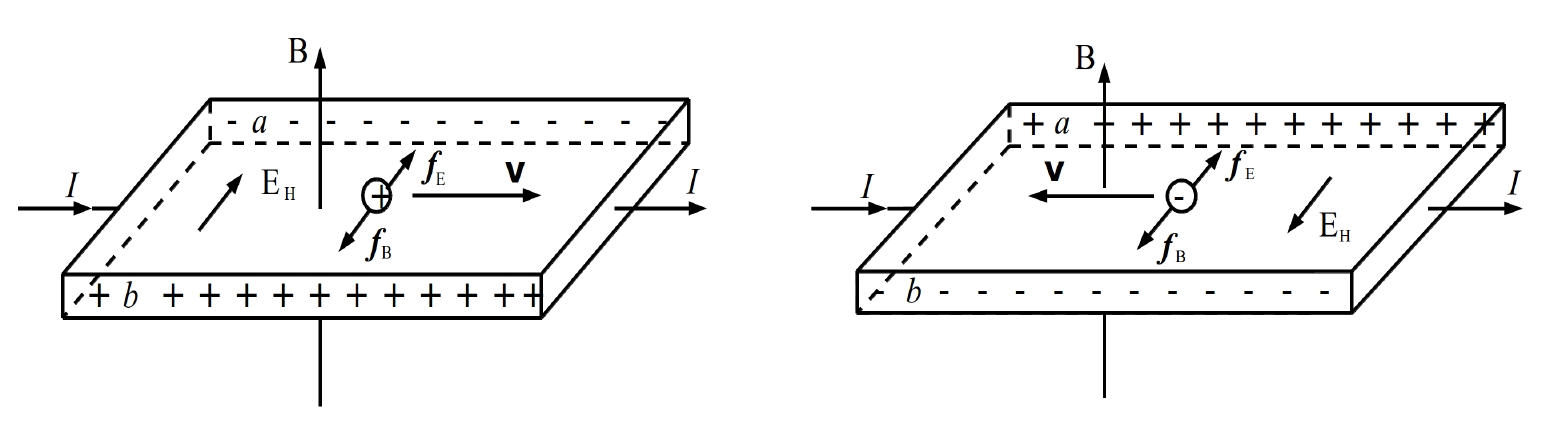
\includegraphics[scale=0.7]{principle.png}
\caption{The principle of the Hall effect.}\label{FigPrinciple}
\end{figure}


	\subsection{Integrated Hall Probe}

However, the Hall voltage is usually very small, it should be amplified before the measurement. An integrated Hall probe, consisting of a Hall sensor, an amplifier, and a voltage compensator (Figure \ref{FigCircuit}), can realize such functions. Hall probe satisfies the following equation:
\begin{equation}\label{eqB}
B = \frac{U-U_0}{K_\text{H}}
\end{equation}
where $U_0$ is the output voltage when the magnetic field is zero.

\begin{figure}[H]
\centering
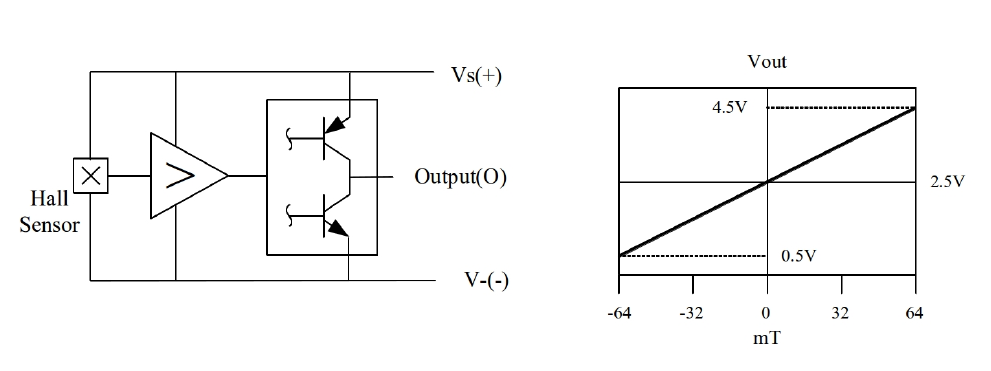
\includegraphics[scale=1.0]{circuit.png}
\caption{The integrated Hall probe SS495A (left). The relation between the output voltage $U$ and the magnitude of the magnetic field $B$ (right).}\label{FigCircuit}
\end{figure}

	\subsection{Magnetic Field Distribution Inside a Solenoid}
Solenoid is a typical electromagnetic element. In this exercise we explore the magnetic field distribution of it with the Hall probe. The theoretical value of magnetic field distribution on the axis of a single layer solenoid can be calculated from the following formula:
\begin{equation}\label{eqBx}
B(x) = \mu_0\frac{N}{L}I_\text{M}\{\frac{L+2x}{2[D^2+(L+2x)^2]^{\frac{1}{2}}}+\frac{L-2x}{2[D^2+(L-2x)^2]^{\frac{1}{2}}}\} = C(x)I_\text{M},
\end{equation}
where $N$ is the number of turns of the solenoid, $L$ is its length, $I_\text{M}$ is the current through the solenoid wire, and D is the solenoid’s diameter. The magnetic permeability of vacuum is $\mu_0 = 4\pi \times 10^{-7} \text{H}/\text{m}.$

The solenoid used in this exercise has ten layers, and the magnetic field $B(x)$ for each layer can be calculated using Eq. (\ref{eqBx}). Then the net magnetic on the axis of the solenoid can be found by adding contributions due to all layers. The theoretical value of the magnetic field inside the solenoid with $I_\text{M}$ = 0.1 A is given in Table \ref{TableTheoB}.

\begin{table}[H]
\centering
\begin{tabular}{cc||cc}
\toprule
$x$ [cm] & $B$ [mT] & $x$ [cm] & $B$ [mT]\\
\hline
$\pm$ 0.0 & 1.4366 & $\pm$ 8.0 & 1.4057\\
$\pm$ 1.0 & 1.4363 & $\pm$ 9.0 & 1.3856\\
$\pm$ 2.0 & 1.4356 & $\pm$ 10.0 & 1.3478\\
$\pm$ 3.0 & 1.4343 & $\pm$ 11.0 & 1.2685\\
$\pm$ 4.0 & 1.4323 & $\pm$ 11.5 & 1.1963\\
$\pm$ 5.0 & 1.4292 & $\pm$ 12.0 & 1.0863\\
$\pm$ 6.0 & 1.4245 & $\pm$ 12.5 & 0.9261\\
$\pm$ 7.0 & 1.4173 & $\pm$ 13.0 & 0.7233\\
\bottomrule
\end{tabular}
 \caption{Theoretical value of the magnetic field inside the solenoid.}\label{TableTheoB}
\end{table}



		\section{Experimental Setup}

The experimental setup (Figure \ref{FigSetup}) consists of an integrated Hall probe SS495A (Figure \ref{FigProbe}) with $K_\text{H}$ = 31.25 $\pm$ 1.25 V/T (at the working voltage 5$\,$V) or $K_\text{H} = 3.125\pm0.125$ mV/G, a solenoid, a power supply, a voltmeter, a DC voltage divider, and a set of connecting wires.

\begin{figure}[H]
\centering
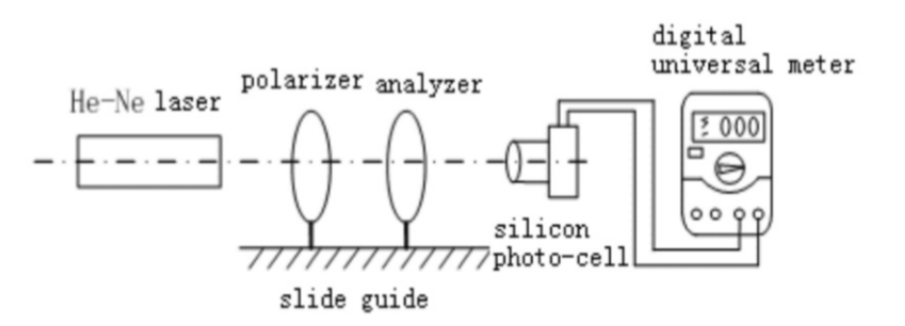
\includegraphics[scale=1.0]{setup.png}
\caption{Measurement setup.}\label{FigSetup}
\end{figure}

\begin{figure}[H]
\centering
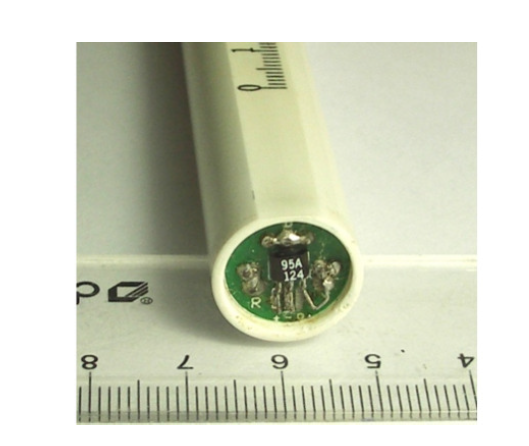
\includegraphics[scale=1.0]{probe.png}
\caption{Measurement setup.}\label{FigProbe}
\end{figure}

The precisions of the devices are shown in Table \ref{tablePrecision}.
\begin{table}[htbp]
\centering
\begin{tabular}{ccc}
\toprule
Instrument & Measured quantities & Uncertainties \\ 
\hline
Voltage source & Working voltage $U_{s}$ & $0.5\%\,$V \\ 
Multimeter & Output voltage $U_{0}, U$ & $0.05\% + 6\times 10^{-3}/10^{-4}\,$V \\ 
Current source & Current $I_{0}, I_{M}$ & $2\%\,$mA \\ 
Graduated ruler & Distance & $0.05\,$cm \\
\bottomrule
\end{tabular}
\caption{Information of measurement instruments.}\label{tablePrecision}
\end{table}



		\section{Measurement Procedure}
		
	\subsection{Relation Between Sensitivity $K_\text{H}$ and Working Voltage $U_\text{S}$\label{proc}}
	
In this part, we explored the relation between sensitivity $K_{H}$ and working voltage $U_{S}$ by applying Eq.\eqref{eqB} and measuring the corresponding quantities. 

First, we placed the integrated Hall probe at the center of the solenoid. Then we set the working voltage at 5 V and measured the output voltage $U_0$ ($I_\text{M}$ = 0) and $U$ ($I_\text{M}$ = 250 mA). We also took the theoretical value of $B(x = 0)$ from Table \ref{TableTheoB} and calculated the sensitivity of the probe $K_\text{H}$ by using Eq. (\ref{eqB}).
Then we measured $K_\text{H}$ for different values of $U_\text{S}$ (from 2.5 V to 10 V). Then we calculated $K_\text{H}/U_\text{S}$ and plotted the curve $K_\text{H}/U_\text{S}$ vs. $U_\text{S}$.


	\subsection{Relation Between Output Voltage $U$ and Magnetic Field $B$}

In this part, we explored the relation between the output voltage of the Hall probe and the magnetic field in which it is positioned by adjusting the current in the solenoid.

First, with $B=0$, $U_\text{S}$ = 5 V, we connected the 2.4 $\sim$ 2.6 V output terminal of the DC voltage divider and the negative port of the voltmeter and adjusted the voltage until $U_0$ = 0.
Next, we placed the integrated Hall probe at the center of the solenoid and measured the output voltage $U$ for different values of $I_\text{M}$ ranging from 0 to 500 mA, with intervals of 50 mA.
Noticing the fact that the output voltage $U$ is the amplified signal from $U_\text{H}$, I tried to explain the relation between $B(x = 0)$ and the Hall voltage $U_\text{H}$.
Then the curve $U$ vs. $B$ is plotted and the sensitivity $K_\text{H}$ is found out.The value is compared with the theoretical value given in the Apparatus section.

	\subsection{Magnetic Field Distribution Inside the Solenoid}

In this part, we explore the magnetic field distribution inside a solenoid by adjusting the position of the Probe Hall and measuring the magnetic field at different positions.

The current in the solenoid is fixed to be $I_\text{M}$ = 250 mA, and thus the magnetic field distribution is fixed. Then the position of the Probe Hall is adjusted and the output voltage $U$ and the corresponding position $x$ are recorded.
Then the curve $B = B(x)$ is plotted and compared with the theoretical value.



		\section{Results}
		
	\subsection{Relation Between Sensitivity $K_\text{H}$ and Working Voltage $U_\text{S}$}
	
The measurement results of $U_0$ and $U$ when $U_\text{S}$ = 5.00 V are shown in Table \ref{TableU5}.

\begin{table}[H]
\centering
\begin{tabular}{ccc}
\toprule
$U_\text{S} \,\,[\text{V}] \pm 0.5\%\,\,[\text{V}]$ & $U_0 (I_\text{M} = 0) \,\,[\text{V}] \pm (0.05\% + 6\times10^{-3} )\,\,[\text{V}]$ & $U (I_\text{M} = 250\,\text{mA}) \,\,[\text{V}] \pm (0.05\% + 6\times10^{-3}) \,\,[\text{V}]$\\
\hline
5.00 $\pm$ 0.03 & 2.476 $\pm$ 0.007 & 2.596 $\pm$ 0.007\\
\bottomrule
\end{tabular}
\caption{Data for $U_0$ and $U$ with $U_\text{S}$ = 5.00 V.}\label{TableU5}
\end{table}

According to the data in Table \ref{TableTheoB}, we can obtain that when $I_\text{M} = 100 \,\,\text{mA},$ $B(x=0,I_\text{M}=100\,[\text{mA}])=1.4366\times10^{-3}\,\,\text{T}.$
Eq. (\ref{eqBx}) implies that $B$ is proportional to current $I_\text{M}$, and therefore, 
$$B(x=0,I_\text{M}=250\,[\text{mA}]) = \frac{250}{100} \times 1.4366\times10^{-3} = 3.5915\times 10^{-3}\,\,\text{T}.$$
According to Eq. (\ref{eqB}), the sensitivity of the probe $K_\text{H}$ when $U_\text{S}$ = 5.00 V is then calculated as 
$$K_\text{H} = \frac{U-U_0}{B(x=0,I_\text{M}=250\,[\text{mA}])} = \frac{2.596-2.476}{3.5915\times 10^{-3}} = 33.412 \pm 2.756 \,[\text{V}/\text{T}].$$

The measurement results of $U_0$ and $U$ for different $U_\text{S}$ are shown in Table \ref{TableK}. We calculate $K_\text{H}/U_\text{S}$ for each set of data to explore their relation. That is, for each set of data, we calculate
$$\displaystyle \frac{K_\text{H}}{U_\text{S}} = \frac{U-U_0}{BU_\text{S}}.$$
Taking the first set of data as an example,
$$\frac{K_\text{H}}{U_\text{S}} = \frac{U-U_0}{BU_\text{S}} = \frac{1.4519-1.3821}{3.5915\times 10^{-3}\times2.80} =  6.9 \pm 0.2 \,[\text{T}^{-1}].$$
The measurement results and the results of calculation of $K_\text{H}/U_\text{S}$ for each set of data are presented together in Table \ref{TableK}. A plot of the results $K_\text{H}/U_\text{S}$ vs. $U_\text{S}$ using Origin is shown in Figure \ref{FigKU}.
The points in the plot indicates that the ratio of $K_{H}$ to $U_{s}$ decreases as $U_{s}$ increases.

\begin{table}[htbp]
\centering
\begin{tabular}{ccccc}
\toprule
& $U_\text{S} \,\,[\text{V}] \pm 0.5\%\,\,[\text{V}]$ & $U_0 \,\,[\text{V}] \pm (0.05\% + 6\times10^{-3/-4}\,\,[\text{V}]$ & $U \,\,[\text{V}] \pm(0.05\% + 6\times10^{-3/-4}\,\,[\text{V}]$ & $K_\text{H}/U_\text{S} \,\,[\text{T}^{-1}]$ \\
\midrule
1 & 2.80 $\pm$ 0.014 & 1.3821 $\pm$ 0.0013 & 1.4519 $\pm$ 0.0013 & 6.9 $\pm$ 0.2\\
2 & 3.20 $\pm$ 0.016 & 1.5817 $\pm$ 0.0014 & 1.6621 $\pm$ 0.0014 & 7.0 $\pm$ 0.2\\
3 & 3.60 $\pm$ 0.018 & 1.7811 $\pm$ 0.0015 & 1.8699 $\pm$ 0.0015 & 6.9 $\pm$ 0.2\\
4 & 4.00 $\pm$ 0.020 & 1.9795 $\pm$ 0.0016 & 2.0806 $\pm$ 0.0016 & 7.0 $\pm$ 0.2\\
5 & 4.40 $\pm$ 0.022 & 2.1793 $\pm$ 0.0017 & 2.286  $\pm$ 0.007 & 6.8 $\pm$ 0.5\\
6 & 4.80 $\pm$ 0.024 & 2.375 $\pm$ 0.007 & 2.491 $\pm$ 0.007 & 6.7 $\pm$ 0.6\\
7 & 5.20 $\pm$ 0.026 & 2.576 $\pm$ 0.007 & 2.697 $\pm$ 0.007 & 6.5 $\pm$ 0.5\\
8 & 5.60 $\pm$ 0.028 & 2.770 $\pm$ 0.007 & 2.900 $\pm$ 0.007 & 6.5 $\pm$ 0.5\\
9 & 6.00 $\pm$ 0.030 & 2.966 $\pm$ 0.007 & 3.100 $\pm$ 0.008 & 6.2 $\pm$ 0.5\\
10 & 6.40 $\pm$ 0.032 & 3.166 $\pm$ 0.008 & 3.306 $\pm$ 0.008 & 6.1 $\pm$ 0.5\\
11 & 6.80 $\pm$ 0.034 & 3.358 $\pm$ 0.008 & 3.501 $\pm$ 0.008 & 5.9 $\pm$ 0.5\\
12 & 7.20 $\pm$ 0.036 & 3.522 $\pm$ 0.008 & 3.699 $\pm$ 0.008 & 6.8 $\pm$ 0.4\\
13 & 7.60 $\pm$ 0.038 & 3.749 $\pm$ 0.008 & 3.895 $\pm$ 0.008 & 5.3 $\pm$ 0.4\\
14 & 8.00 $\pm$ 0.040 & 3.943 $\pm$ 0.008 & 4.092 $\pm$ 0.008 & 5.2 $\pm$ 0.4\\
15 & 8.40 $\pm$ 0.042 & 4.136 $\pm$ 0.008 & 4.286 $\pm$ 0.008 & 5.0 $\pm$ 0.4\\
16 & 8.80 $\pm$ 0.044 & 4.327 $\pm$ 0.008 & 4.480 $\pm$ 0.008 & 4.8 $\pm$ 0.4\\
17 & 9.20 $\pm$ 0.046 & 4.525 $\pm$ 0.008 & 4.682 $\pm$ 0.008 & 4.8 $\pm$ 0.3\\
18 & 9.60 $\pm$ 0.048 & 4.710 $\pm$ 0.008 & 4.868 $\pm$ 0.008 & 4.6 $\pm$ 0.3\\
\bottomrule
\end{tabular}
\caption{Data for $U_0$, $U$ and $K_\text{H}/U_\text{S}$ for different $U_\text{S}$.}\label{TableK}
\end{table}

\begin{figure}[H]
\centering
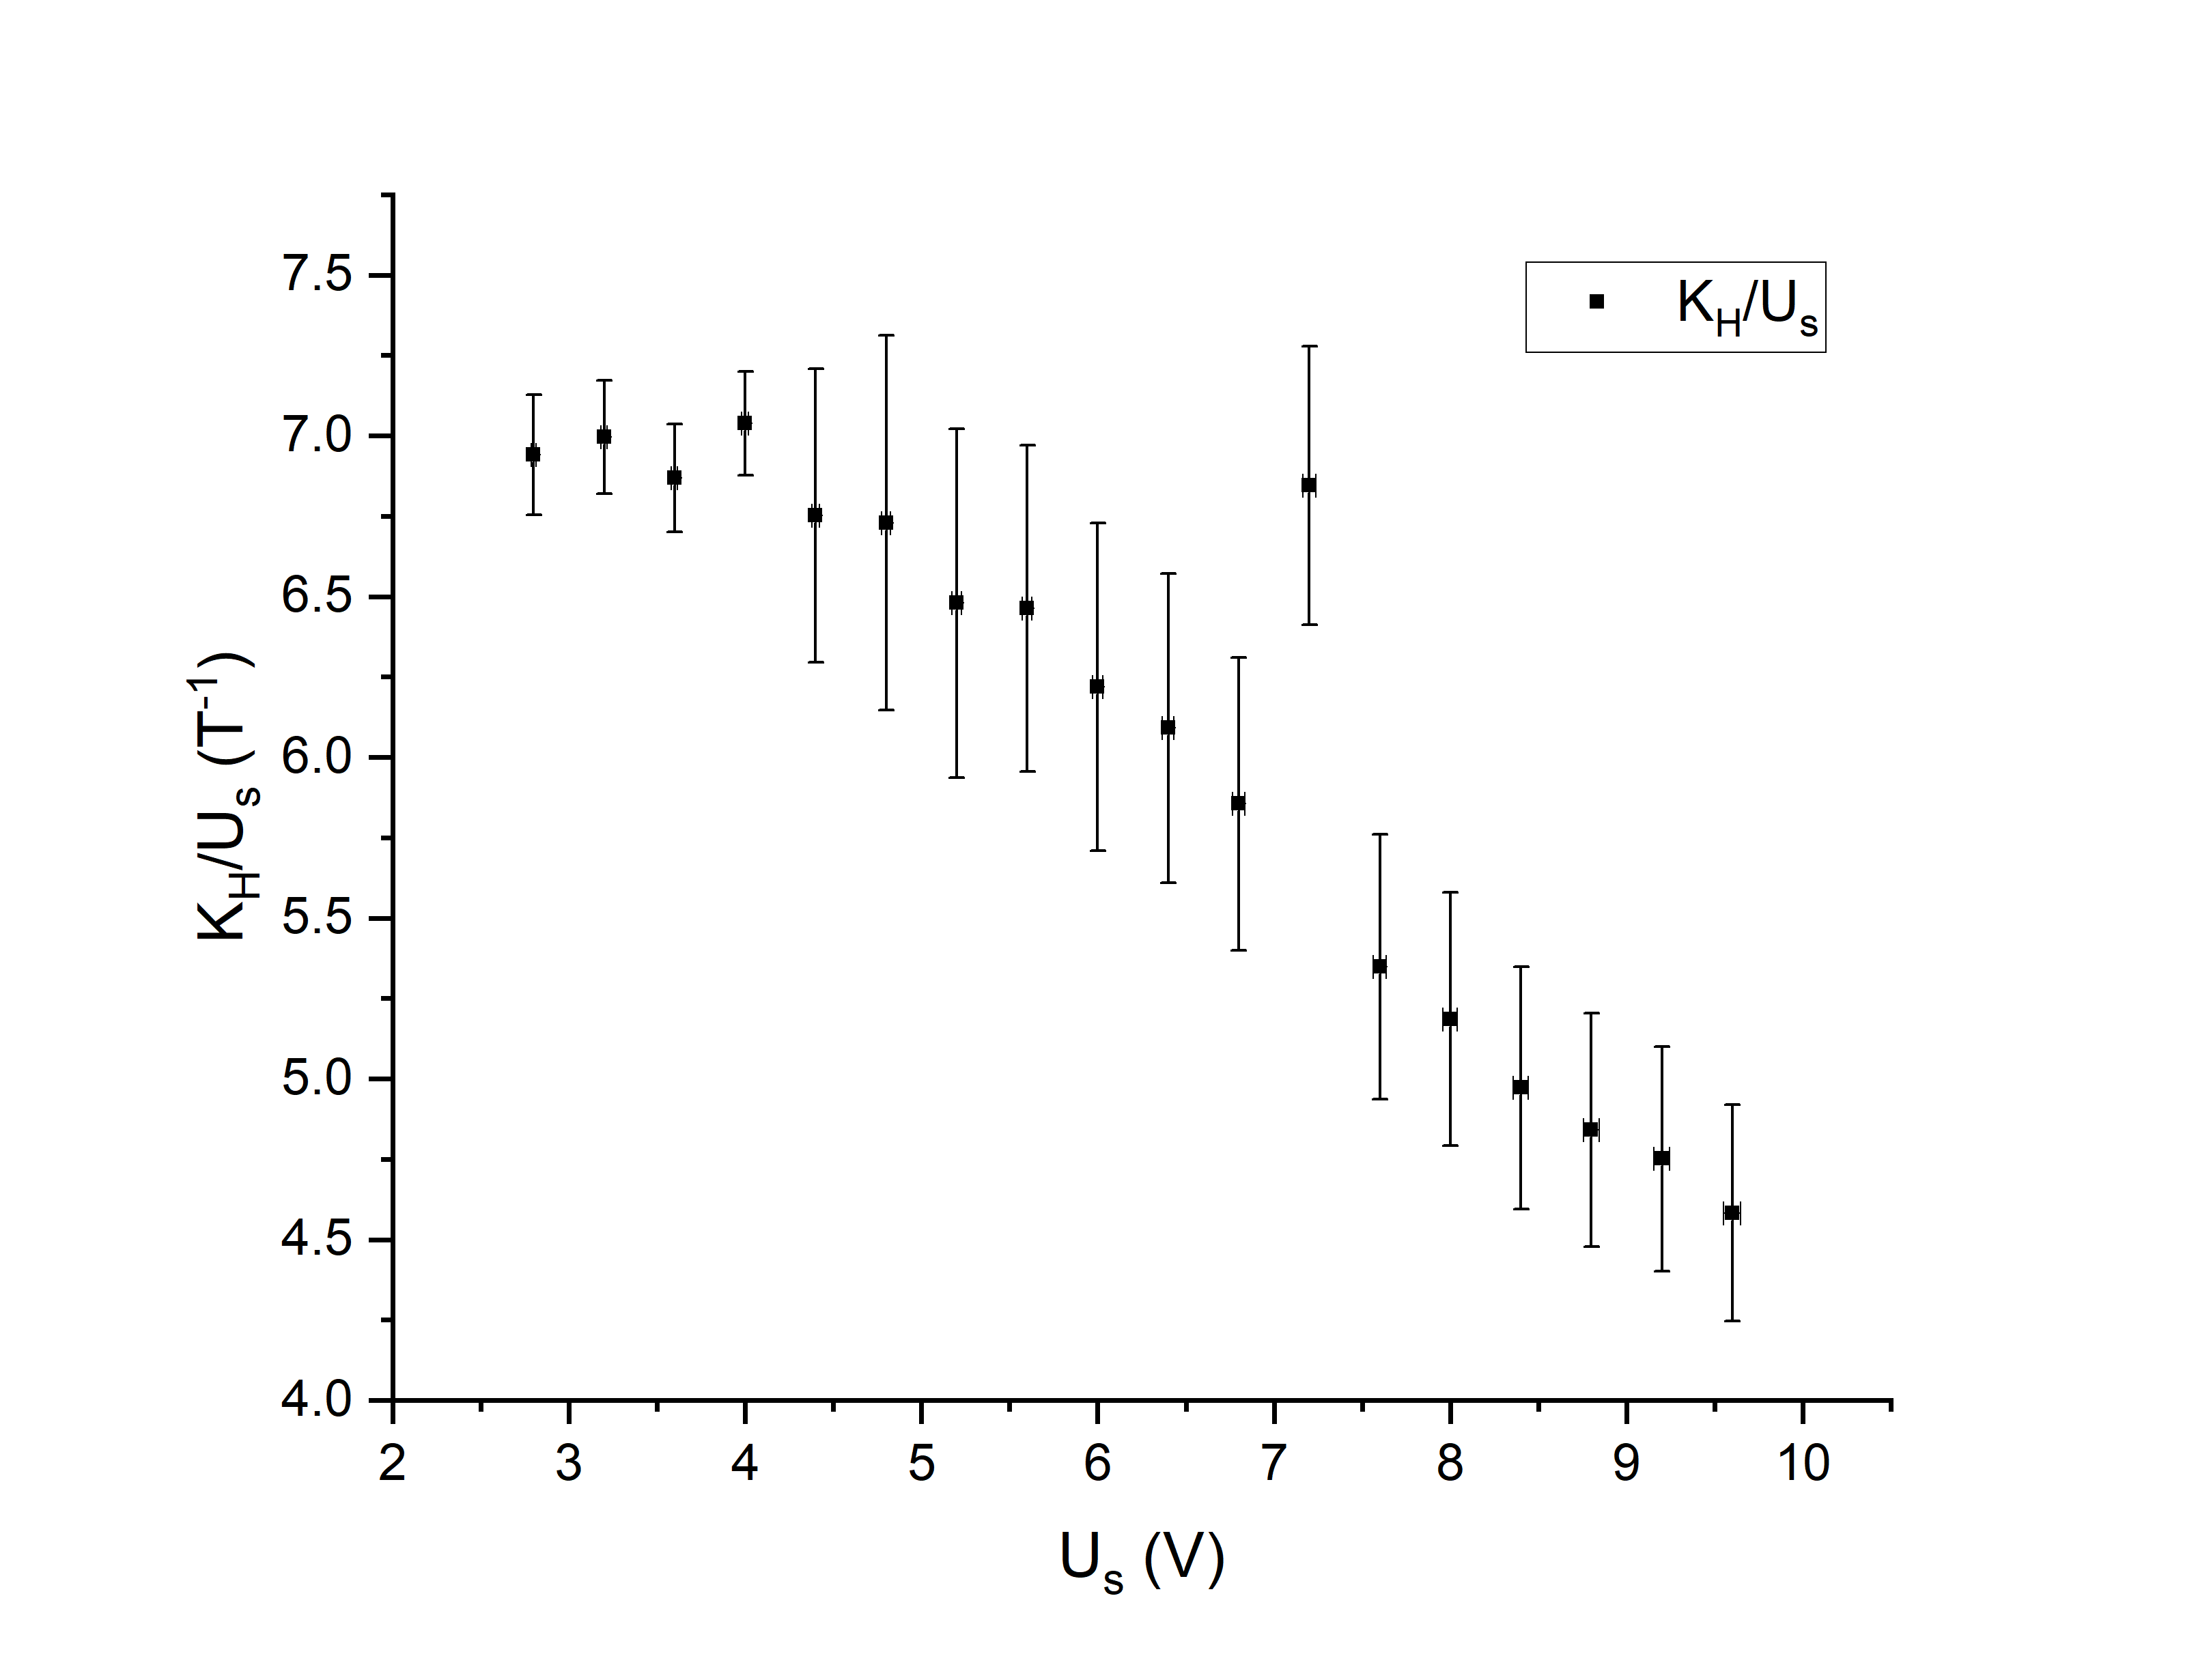
\includegraphics[scale=0.4]{plot1.png}
\caption{The $K_\text{H}/U_\text{S}$ vs. $U_\text{S}$ relation.}\label{FigKU}
\end{figure}

	\subsection{Relation Between Output Voltage $U$ and Magnetic Field $B$}\label{SecUB}
	
According to Eq. (\ref{eqBx}), $B$ is proportional to current $I_\text{M}$. We can obtain from Table \ref{TableTheoB} that when $I_\text{M} = 100 \,\,\text{mA},$ $B(x=0,I_\text{M}=100\,[\text{mA}])=1.4366\times10^{-3}\,\,\text{T}.$ Therefore, 
the theoretical value of the magnetic field is $$B(x=0) = \frac{I_\text{M}}{100}\times 1.4366\times10^{-3}.$$
Take the second set of data as an example, 
$$B(x=0,I_\text{M}=50\,[\text{mA}]) = \frac{1.4366\times10^{-3}}{50}\times I_\text{M} = 0.718\times 10^{-3}\,[\text{T}].$$

It is noticed that the measured $U$ is the amplified output of $U_{H}$ and we supposed that $U = k \cdot U_{H}$. Then, theoretically, according to Eq. (\ref{eqB}), we can derive that
$$B(x=0) = \frac{U-U_0}{K_\text{H}} = \frac{U}{K_\text{H}} = k\cdot\frac{U_\text{H}}{K_\text{H}},$$
where $k$ is a constant. Therefore, $B(x=0)$ is supposed to be proportional to the Hall voltage $U_\text{H}$.\\

The experimental results are shown in Table \ref{TableI}. By applying linear fit to the $I_\text{M}$ vs. $U$ plot (Figure \ref{FigUB}), the slope of the curve is then the measured sensitivity $K_{H}$, which is $ 0.03197 / 10^{-3} = 31.97\,$V/T, with uncertainty $6 \times 10^{-4} / 10^{-3} = 0.6\,$V/T. The measurement result of the sensitivity is then $K_H = 32.0 \pm 0.6\,$V/T.

\begin{table}[H]
\centering
\begin{tabular}{cccc}
\toprule
& $I_\text{M}\,\,[\text{A}] \pm 2\%\,\,[\text{A}]$ & $B(x=0)\,\,[10^{-3}\,\text{T}]$ & $U\,\,[\text{V}]\pm (0.05\%+6\times10^{-3/-4})\,\,[\text{V}]$\\
\midrule
1 & 0 $\pm$ 0  & 0 $\pm$ 0 & 0.000 $\pm$ 0.0006 \\
2 & 0.050 $\pm$ 0.001 & 0.718 $\pm$ 0.014 & 0.02855 $\pm$ 0.0006 \\
3 & 0.100 $\pm$ 0.02 & 1.44 $\pm$ 0.03 & 0.05004 $\pm$ 0.0006 \\
4 & 0.150 $\pm$ 0.03 & 2.16 $\pm$ 0.04 & 0.07532 $\pm$ 0.0006 \\
5 & 0.200 $\pm$ 0.04 & 2.87 $\pm$ 0.06 & 0.09897 $\pm$ 0.0006 \\
6 & 0.250 $\pm$ 0.05 & 3.59 $\pm$ 0.07 & 0.1182 $\pm$ 0.0006 \\
7 & 0.300 $\pm$ 0.06 & 4.31 $\pm$ 0.09 & 0.14301 $\pm$ 0.0006 \\
8 & 0.350 $\pm$ 0.07 & 5.03 $\pm$ 0.10 & 0.16314 $\pm$ 0.0006 \\
9 & 0.400 $\pm$ 0.08 & 5.75 $\pm$ 0.11 & 0.18792 $\pm$ 0.0006 \\
10 & 0.450 $\pm$ 0.09 & 6.47 $\pm$ 0.13 & 0.21184 $\pm$ 0.0006 \\
11 & 0.500 $\pm$ 0.10 & 7.18 $\pm$ 0.14 & 0.2319 $\pm$ 0.0006 \\
\bottomrule
\end{tabular}
\caption{Measurement data for the $I_\text{M}$ vs. $U$ relation and the calculated data for $B(x=0)$.}\label{TableI}
\end{table}

\begin{figure}[H]
\centering
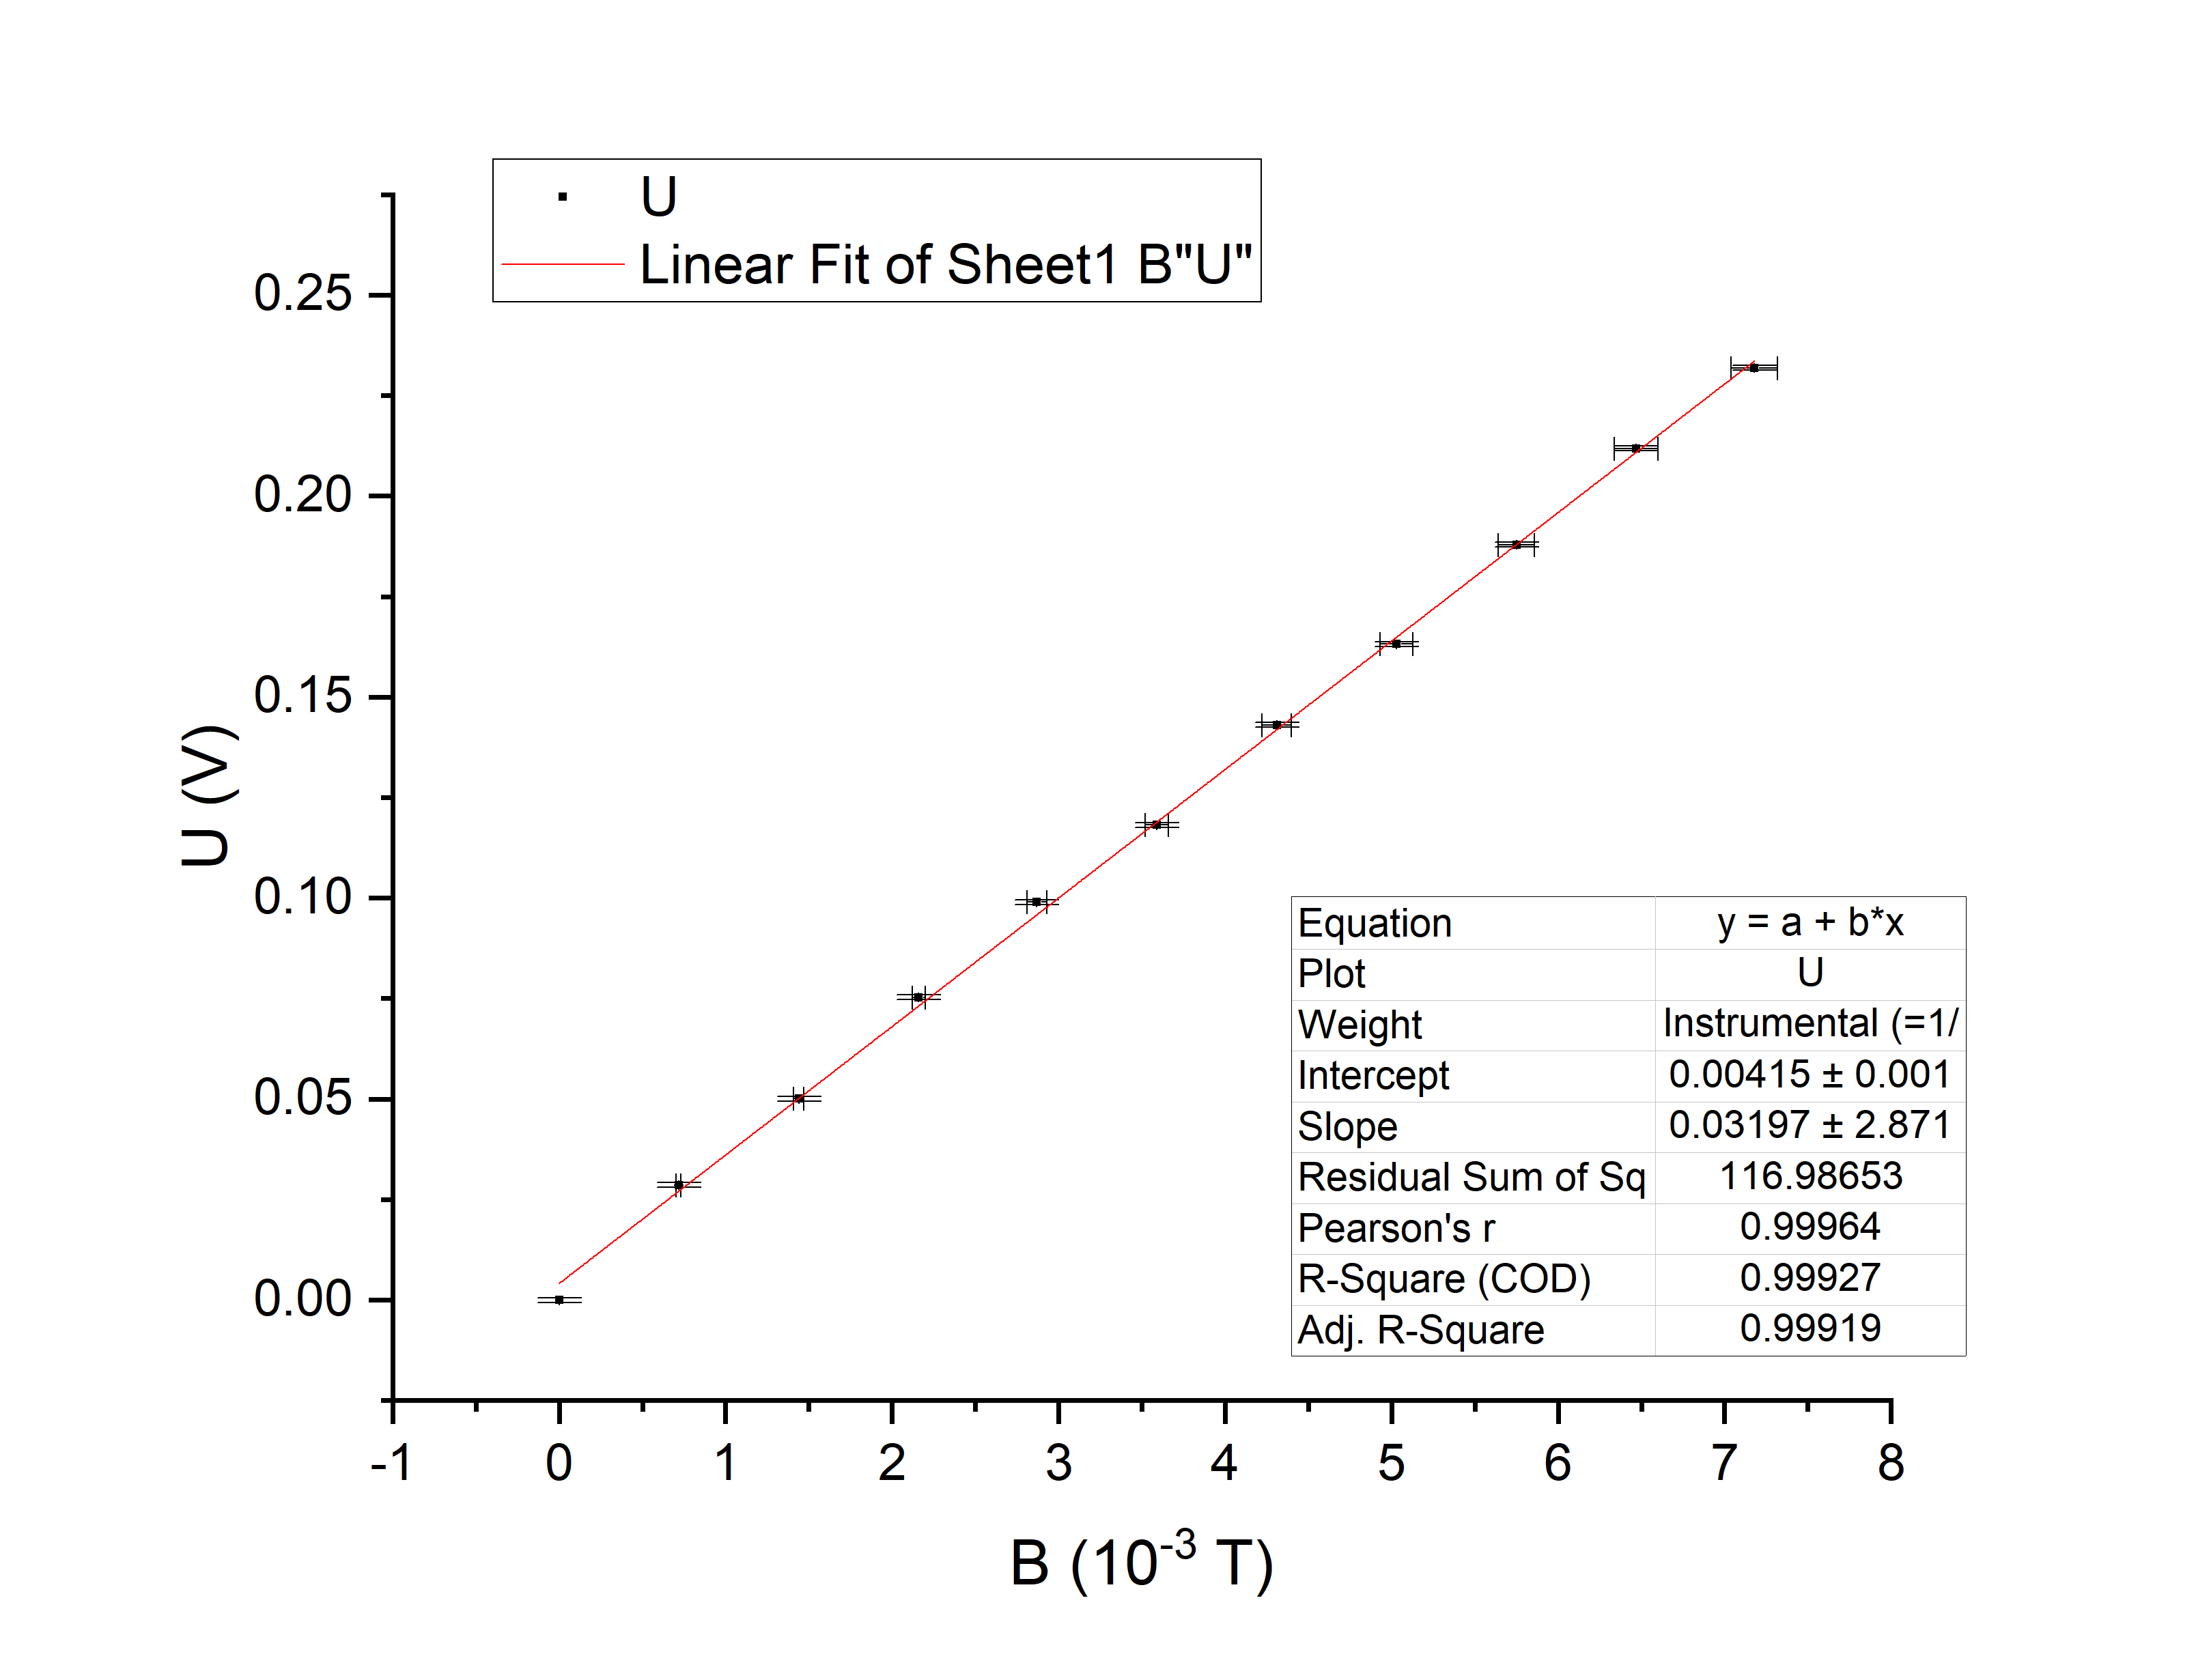
\includegraphics[scale=0.4]{plot2.png}
\caption{The linear fit of $U$ vs. $B$ relation.}\label{FigUB}
\end{figure}

	\subsection{Magnetic Field Distribution Inside the Solenoid}

The measurement result of output voltage $U$ and the corresponding position $x$ are shown in Table \ref{TableUx}. According to Eq.\eqref{eqB} and the measured value of $K_{H}$ in section \ref{SecUB}, $B(x)$ can be obtained from $\displaystyle B(x) = \frac{U}{K_\text{H}} = \frac{U}{32.0} .$
Take the first set of data as an example, $$B(x) = \frac{U}{32.0} = \frac{0.00961}{32.0} = (0.30 \pm 0.02) \times 10^{-3} \,\,[\text{T}].$$ 
The $B(x)$ are calculated for each set of data and the results are shown in Table \ref{TableBx}.

\begin{table}[htbp]
\centering
\begin{tabular}{ccc||ccc}
\toprule
& $x$[cm]$\pm$0.05[cm] & $U$[V]$\pm$(0.05$\%$+$6 \times 10^{-4})[\text{V}]$ & & $x$[cm]$\pm$0.05[cm] & $U$[V]$\pm$(0.05$\%$+$6 \times 10^{-4})[\text{V}]$\\
\midrule
    1     & 0    & 0.0096 $\pm$ 0.0006 & 27    & 15.3  & 0.1195 $\pm$ 0.0006 \\
    2     & 0.2  & 0.0110 $\pm$ 0.0006 & 28    & 16.3  & 0.1196 $\pm$ 0.0006 \\
    3     & 0.4  & 0.0121 $\pm$ 0.0006 & 29    & 17.3  & 0.1196 $\pm$ 0.0006 \\
    4     & 0.6  & 0.0136 $\pm$ 0.0006 & 30    & 18.3  & 0.1195 $\pm$ 0.0006 \\
    5     & 0.8  & 0.0158 $\pm$ 0.0006 & 31    & 19.3  & 0.1194 $\pm$ 0.0006 \\
    6     & 1    & 0.0180 $\pm$ 0.0006 & 32    & 20.3  & 0.1190 $\pm$ 0.0006 \\
    7     & 1.3  & 0.0218 $\pm$ 0.0006 & 33    & 21.2  & 0.1187 $\pm$ 0.0006 \\
    8     & 1.6  & 0.0164 $\pm$ 0.0006 & 34    & 22.1  & 0.1183 $\pm$ 0.0006 \\
    9     & 2.1  & 0.0397 $\pm$ 0.0006 & 35    & 22.9  & 0.1178 $\pm$ 0.0006 \\
    10    & 2.5  & 0.0523 $\pm$ 0.0006 & 36    & 23.7  & 0.1169 $\pm$ 0.0006 \\
    11    & 3    & 0.0694 $\pm$ 0.0006 & 37    & 24.4  & 0.1159 $\pm$ 0.0006 \\
    12    & 3.6  & 0.0873 $\pm$ 0.0006 & 38    & 25.1  & 0.1140 $\pm$ 0.0006 \\
    13    & 1.2  & 0.0996 $\pm$ 0.0006 & 39    & 25.8  & 0.1117 $\pm$ 0.0006 \\
    14    & 1.9  & 0.1069 $\pm$ 0.0006 & 40    & 26.4  & 0.1084 $\pm$ 0.0006 \\
    15    & 5.6  & 0.1117 $\pm$ 0.0006 & 41    & 27    & 0.1026 $\pm$ 0.0006 \\
    16    & 6.3  & 0.1143 $\pm$ 0.0006 & 42    & 27.5  & 0.0951 $\pm$ 0.0006 \\
    17    & 7.1  & 0.1163 $\pm$ 0.0006 & 43    & 27.9  & 0.0863 $\pm$ 0.0006 \\
    18    & 7.9  & 0.1174 $\pm$ 0.0006 & 44    & 28.4  & 0.0709 $\pm$ 0.0006 \\
    19    & 8.8  & 0.1182 $\pm$ 0.0006 & 45    & 28.7  & 0.0590 $\pm$ 0.0006 \\
    20    & 9.7  & 0.1187 $\pm$ 0.0006 & 46    & 29    & 0.0496 $\pm$ 0.0006 \\
    21    & 10.7 & 0.1191 $\pm$ 0.0006 & 47    & 29.2  & 0.0432 $\pm$ 0.0006 \\
    22    & 11.7 & 0.1194 $\pm$ 0.0006 & 48    & 29.4  & 0.0374 $\pm$ 0.0006 \\
    23    & 12.7 & 0.1195 $\pm$ 0.0006 & 49    & 29.6  & 0.0322 $\pm$ 0.0006 \\
    24    & 13.7 & 0.1195 $\pm$ 0.0006 & 50    & 29.8  & 0.0284 $\pm$ 0.0006 \\
    25    & 14.7 & 0.1195 $\pm$ 0.0006 & 51    & 30    & 0.0244 $\pm$ 0.0006 \\
    26    & 15   & 0.1195 $\pm$ 0.0006   \\
\bottomrule
\end{tabular}
\caption{Data for the $U$ vs. $x$ relation}\label{TableUx}
\end{table}

\begin{table}[htbp]
\centering
\begin{tabular}{ccc||ccc}
\toprule
& $x\,\,[\text{cm}] \pm 0.05\,\,[\text{cm}]$ & $B(x)\,\,[10^{-3}\,\,\text{T}]$ & & $x\,\,[\text{cm}] \pm 0.05\,\,[\text{cm}]$ & $B(x)\,\,[10^{-3}\,\,\text{T}]$\\
\midrule
 	1     & 0     & 0.30 $\pm$ 0.02 & 27    & 15.3  & 3.73 $\pm$ 0.07 \\
    2     & 0.2   & 0.34 $\pm$ 0.02 & 28    & 16.3  & 3.74 $\pm$ 0.07 \\
    3     & 0.4   & 0.38 $\pm$ 0.02 & 29    & 17.3  & 3.74 $\pm$ 0.07 \\
    4     & 0.6   & 0.42 $\pm$ 0.02 & 30    & 18.3  & 3.73 $\pm$ 0.07 \\
    5     & 0.8   & 0.49 $\pm$ 0.02 & 31    & 19.3  & 3.73 $\pm$ 0.07 \\
    6     & 1     & 0.56 $\pm$ 0.02 & 32    & 20.3  & 3.72 $\pm$ 0.07 \\
    7     & 1.3   & 0.68 $\pm$ 0.02 & 33    & 21.2  & 3.71 $\pm$ 0.07 \\
    8     & 1.6   & 0.51 $\pm$ 0.02 & 34    & 22.1  & 3.70 $\pm$ 0.07 \\
    9     & 2.1   & 1.24 $\pm$ 0.03 & 35    & 22.9  & 3.68 $\pm$ 0.07 \\
    10    & 2.5   & 1.63 $\pm$ 0.04 & 36    & 23.7  & 3.65 $\pm$ 0.07 \\
    11    & 3     & 2.17 $\pm$ 0.04 & 37    & 24.4  & 3.62 $\pm$ 0.07 \\
    12    & 3.6   & 2.73 $\pm$ 0.05 & 38    & 25.1  & 3.56 $\pm$ 0.07 \\
    13    & 1.2   & 3.11 $\pm$ 0.06 & 39    & 25.8  & 3.49 $\pm$ 0.07 \\
    14    & 1.9   & 3.34 $\pm$ 0.07 & 40    & 26.4  & 3.39 $\pm$ 0.07 \\
    15    & 5.6   & 3.49 $\pm$ 0.07 & 41    & 27    & 3.21 $\pm$ 0.06 \\
    16    & 6.3   & 3.57 $\pm$ 0.07 & 42    & 27.5  & 2.97 $\pm$ 0.06 \\
    17    & 7.1   & 3.63 $\pm$ 0.07 & 43    & 27.9  & 2.70 $\pm$ 0.05 \\
    18    & 7.9   & 3.67 $\pm$ 0.07 & 44    & 28.4  & 2.22 $\pm$ 0.05 \\
    19    & 8.8   & 3.69 $\pm$ 0.07 & 45    & 28.7  & 1.84 $\pm$ 0.04 \\
    20    & 9.7   & 3.71 $\pm$ 0.07 & 46    & 29    & 1.55 $\pm$ 0.03 \\
    21    & 10.7  & 3.72 $\pm$ 0.07 & 47    & 29.2  & 1.35 $\pm$ 0.03 \\
    22    & 11.7  & 3.73 $\pm$ 0.07 & 48    & 29.4  & 1.17 $\pm$ 0.03 \\
    23    & 12.7  & 3.73 $\pm$ 0.07 & 49    & 29.6  & 1.01 $\pm$ 0.03 \\
    24    & 13.7  & 3.73 $\pm$ 0.07 & 50    & 29.8  & 0.89 $\pm$ 0.03 \\
    25    & 14.7  & 3.73 $\pm$ 0.07 & 51    & 30    & 0.76 $\pm$ 0.02 \\
    26    & 15    & 3.73 $\pm$ 0.07 \\
\bottomrule
\end{tabular}
\caption{Data for the $B(x)$ vs. $x$ relation.}\label{TableBx}
\end{table}

The theoretical curve of the magnetic field distribution inside the solenoid can be obtained from Eq.\eqref{eqBx} and the data in Table \ref{TableTheoB}, by multiplying the data in the table by $\frac{250}{100} = 2.5$, since we have set the current as 250 mA instead of 100 mA.

Then we plot the theoretical curve together with the measured value of the magnetic field distribution in Figure \ref{FigB}. The origin of the plot is set at the center of the solenoid, so $13\,cm$ are subtracted from the $x$ in the measurement data.

\begin{figure}[H]\centering
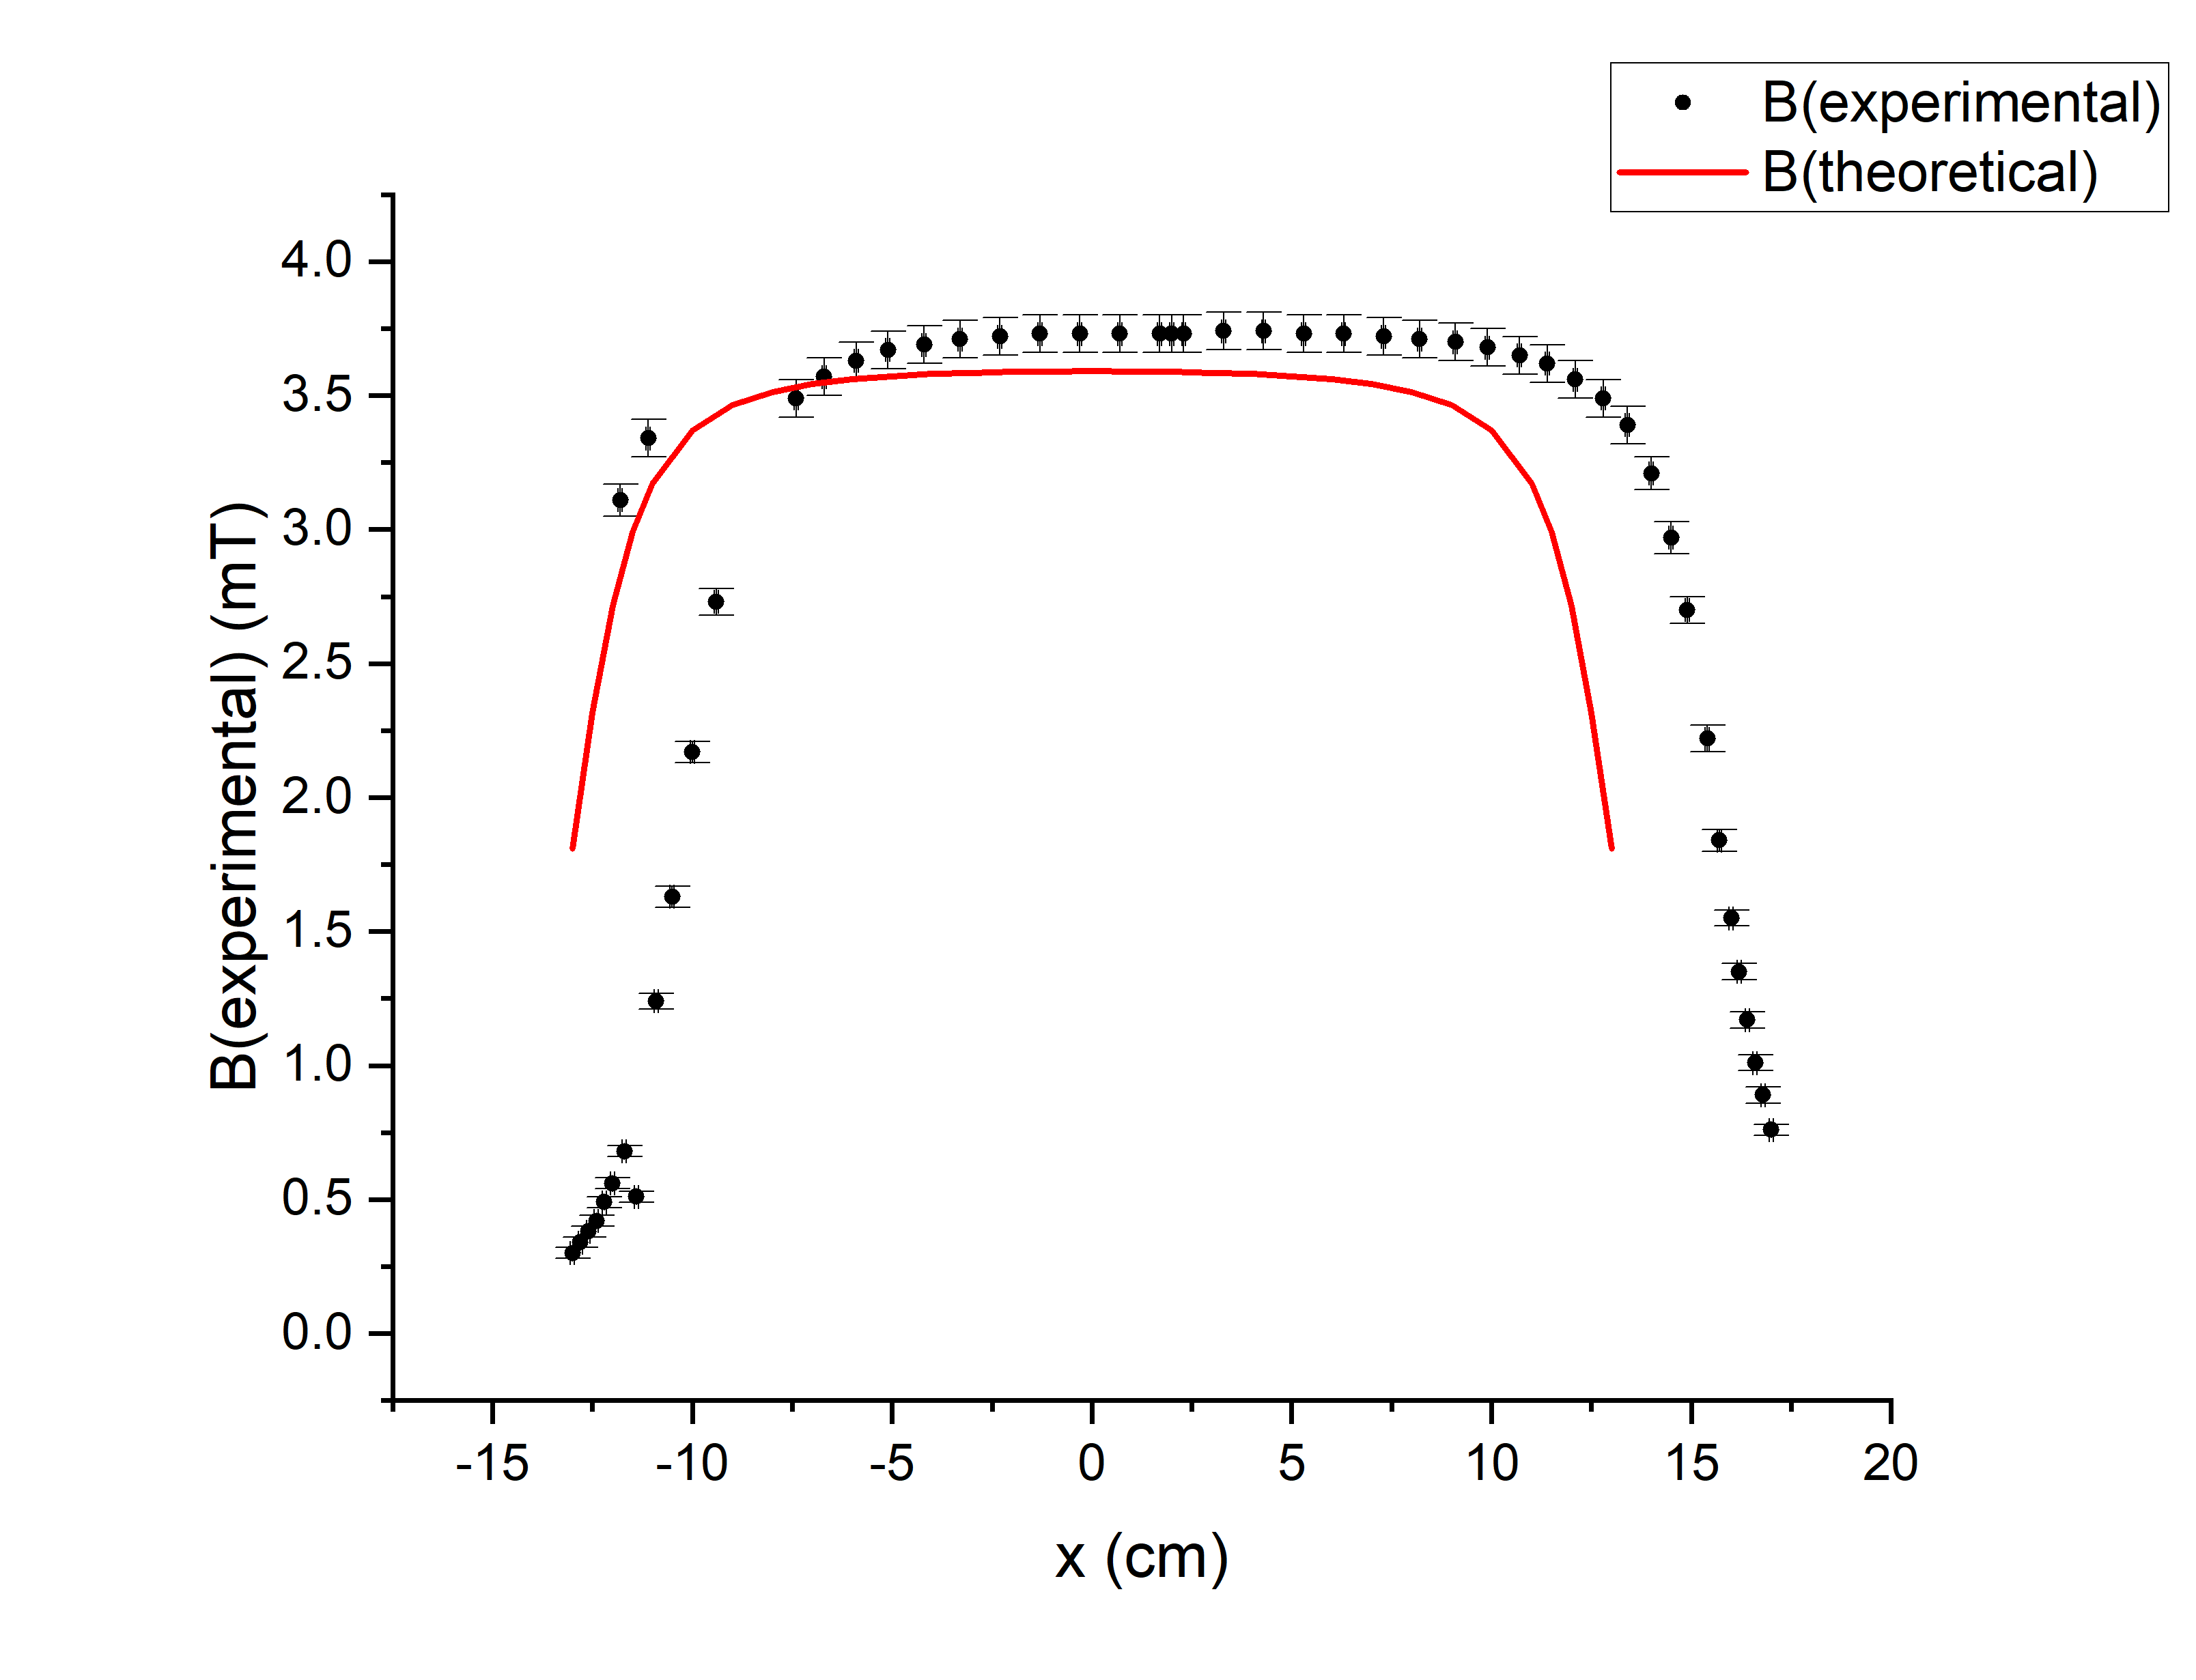
\includegraphics[scale=0.4]{plot3.png}
\caption{Measured and theoretical magnetic field distribution inside the solenoid.}\label{FigB}
\end{figure}



		\section{Conclusions and Discussion}
		
	\subsection{Relation Between Sensitivity $K_\text{H}$ and Working Voltage $U_\text{S}$}

From Figure \ref{FigKU}, the results of my experiment implies that the sensitivity decreases as working voltage increases.

However, theoretically, the sensitivity should increase as the working voltage does [1]. After searching for information, one reason that I come up with is that the temperature affects the sensitivity. As presented in [1], the sensitivity of SS495 increases significantly enough to affect the experimental result as temperature increases. 
 
In view of this, I suggest that temperature should be controlled when conducting this experiment, that is, we turn on the current source for a short time and perform one or two set of measurement, and then cut the source, wait for a while and then turn on the source again to continue with the measurement.
	
	\subsection{Relation Between Output Voltage $U$ and Magnetic Field $B$}
	
In this part, the Pearson's r of the fitting is 0.99964, which implies that the output voltage is most likely to be linearly dependent on the magnetic field. Since the output voltage is 0 when magnetic field is zero, then we can deduce that the output voltage is proportional to the magnetic field.

Besides, the sensitivity we obtained from the plot is 32.0 V/T, this compares with the theoretical value 31.25 [1], with relative error
$$U_{rK_\text{H}} = \frac{32.0-31.25}{31.25}\times 100\% = 2.4\,\%.$$
The experimental results agrees with the actual value.

One possible cause for the inaccuracy of the experiment is that Eq.\eqref{FigUB} holds only "when the external magnetic field is not too strong" [2]. In this part, the current has been adjusted to up to 500 mA, which may result in non-proportional relation. Another cause may be that the input voltage of the amplifier exceeds the saturation value of the amplifier, which results in the inaccuracy of the output voltage.
	
	
	
	\subsection{Magnetic Field Distribution Inside the Solenoid}
	
It can be seen from Figure \ref{FigB} that the experimental value does not match the theoretical value in a satisfying range. However, it is observed that the theoretical curve can be obtained by moving the experimental curve to the left a little bit, ignoring the two obviously wrong sets of data. Inspired by this, I guess that one possible reason of the discrepancy  is that the scale solenoid is inaccurate.

Despite the inaccuracy of our result, the variation trend of the curve agrees with the theoretical trend. The magnetic field increases rapidly as the distance from the center becomes smaller. After it reaches its maximum, it becomes nearly constant.

\vspace{0.5cm}

Some other comments and suggestions are also listed below:
\begin{enumerate}
\item The data displayed on the device is not stable, and we had to choose one data to record, which can lead to error. It is suggested that using apparatus of higher accuracy can reduce the uncertainty and inaccuracy of the experiment.
\item Generally, the magnetic field of the earth may affect the whole experiment.
\end{enumerate}



		\section{Reference}

\noindent [1] Specifications of SS495 provided by Honeywell Sensing and Control, posted on www.umjicanvas.com VP241 2019 Fall.

\noindent [2] VP241 Exercise 2: The hall probe: characteristics and applications, Shanghai Jiaotong University.



\newpage



\appendix



		\section{Measurement Uncertainty Analysis}

	\subsection{Uncertainty of Sensitivity $K_\text{H}$ and Voltage Measurements}

For Table \ref{TableU5}, the uncertainties are calculated as
$$u_{U_\text{S}} = 5.00\times 0.5\% = 0.03\,\,[\text{V}],$$
$$u_{U_0} = 2.476\times0.05\%+6\times10^{-3} = 0.007\,\,[\text{V}],$$
$$u_U = 2.596\times0.05\%+6\times10^{-3} = 0.007\,\,[\text{V}].$$

For $K_\text{H} = \frac{U-U_0}{B}$, its uncertainty is
\begin{align*}
u_{K_\text{H}} &= \sqrt{(\frac{\partial K_\text{H}}{\partial U}u_U)^2+(\frac{\partial K_\text{H}}{\partial U_0}u_{U_0})^2} = \sqrt{(\frac{u_U}{B})^2+(\frac{-u_{U_0}}{B})^2} \\
&=\sqrt{(\frac{0.007}{1.4366\times10^{-3}\times250/100})^2+(\frac{-0.007}{1.4366\times10^{-3}\times250/100})^2} =2.756\,\,[\text{V}/\text{T}].
\end{align*}


For Table \ref{TableK}, the uncertainties of data for voltage measurements are calculated as follows. Take the first set of data as an example, 
$$u_{U_\text{S}} = 2.80\times 0.5\% = 0.014\,\,[\text{V}],$$
$$u_{U_0} = 1.3821\times0.05\%+6\times10^{-4} = 0.0013\,\,[\text{V}],$$
$$u_U = 1.4519\times0.05\%+6\times10^{-4} = 0.0013\,\,[\text{V}].$$

The uncertainty for $ \displaystyle K_\text{H}/U_\text{S} = \frac{U-U_0}{BU_\text{S}}$ is calculated as
\begin{align*}
u_{K_\text{H}/U_\text{S}} &= \sqrt{(\frac{\partial K_\text{H}/U_\text{S}}{\partial U}u_U)^2+(\frac{\partial K_\text{H}/U_\text{S}}{\partial U_0}u_{U_0})^2+(\frac{\partial K_\text{H}/U_\text{S}}{\partial U_\text{S}}u_{U_\text{S}})^2} \\
&= \sqrt{(\frac{u_U}{BU_\text{S}})^2+(\frac{-u_{U_0}}{BU_\text{S}})^2+(-\frac{U-U_0}{BU_\text{S}^2}u_{U_\text{S}})^2} \\
&= \sqrt{(\frac{u_U}{BU_\text{S}})^2+(\frac{-u_{U_0}}{BU_\text{S}})^2+(-\frac{U-U_0}{BU_\text{S}^2}u_{U_\text{S}})^2} \\
&= \sqrt{(\frac{0.0013}{1.4366\times10^{-3}\times250/100\times2.80})^2+(\frac{-0.0013}{1.4366\times10^{-3}\times250/100 \times2.80})^2+(-\frac{1.4519-1.3821}{1.4366\times10^{-3}\times250/100 \times2.80^2}\times0.014)^2} \\
&=0.2\,\,[\text{T}^{-1}].
\end{align*}

The uncertainties of all other data in Table \ref{TableK} are calculated in this way and the results are presented in Table \ref{TableUncK}.

\begin{table}[H]
\centering
\begin{tabular}{crrrc}
\toprule
& $u_{U_\text{S}}\,\,[\text{V}]$ & $u_{U_0}\,\,[\text{V}]$ & $u_U\,\,[\text{V}]$ & $u_{K_\text{H}/U_\text{S}}\,\,[\text{T}^{-1}]$\\
\midrule
  1 & 0.014 & 0.0013 &0.0013 &0.2 \\
  2 & 0.016 & 0.0014 &0.0014 &0.2 \\
  3 & 0.018 & 0.0015 &0.0015 &0.2 \\
  4 & 0.020 & 0.0016 &0.0016 &0.2 \\
  5 & 0.022 & 0.0017& 0.007 & 0.5\\
  6 & 0.024 & 0.007 & 0.007 & 0.6\\
  7 & 0.026 & 0.007 & 0.007 & 0.5\\
  8 & 0.028 & 0.007 & 0.007 & 0.5\\
  9 & 0.030 & 0.007 & 0.008 & 0.5\\
  10 & 0.032 &0.008  &0.008  &0.5 \\
  11 & 0.034 &0.008  &0.008  &0.5 \\
  12 & 0.036 &0.008  &0.008  &0.4 \\
  13 & 0.038 &0.008  &0.008  &0.4 \\
  14 & 0.040 &0.008  &0.008  &0.4 \\
  15 & 0.042 &0.008  &0.008  &0.4 \\
  16 & 0.044 &0.008  &0.008  &0.4 \\
  17 & 0.046 &0.008  &0.008  &0.3 \\
  18 & 0.048 &0.008  &0.008  &0.3 \\
\bottomrule
\end{tabular}
\caption{Uncertainties of data in Table \ref{TableK}.}\label{TableUncK}
\end{table}

	\subsection{Uncertainty of Input Current $I_\text{M}$, Output Voltage $U$ and Magnetic Field $B$}

Take the second set of data in Table \ref{TableI} as an example.\\

The uncertainty for $I_\text{M}$ is
$$u_{I_\text{M}} = 50\times 2\% = 1\,\,[\text{mA}] = 0.001\,\,[\text{A}].$$

The uncertainty for $U$ is 
$$u_U = 0.02855\times 0.05\%+6\times10^{-4} = 0.0006\,\,[\text{V}].$$

The uncertainty for $B = 0.014366 \times I_\text{M}$ is
$$u_B = 0.014366 \times u_{I_\text{M}} = 0.014366 \times 0.001 = 1.4\times 10^{-5}\,\,[\text{T}].$$

The uncertainties of all other data in Table \ref{TableI} are calculated in this way are the results are presented in Table \ref{TableUncI}.

\begin{table}[H]
\centering
\begin{tabular}{cccc}
\toprule
& $u_{I_\text{M}}\,\,[\text{A}]$ & $u_B\,\,[\text{T}]$ & $u_U\,\,[\text{V}]$\\
\midrule
    1     & 0 & 0   & 0.0006 \\
    2     & 0.001 & 0.000014  & 0.0006 \\
    3     & 0.002 & 0.00003  & 0.0006 \\
    4     & 0.003 & 0.00004  & 0.0006 \\
    5     & 0.004 & 0.00006  & 0.0006 \\
    6     & 0.005 & 0.00007  & 0.0006 \\
    7     & 0.006 & 0.00009  & 0.0006 \\
    8     & 0.007 & 0.00010  & 0.0006 \\
    9     & 0.008 & 0.00011  & 0.0006 \\
    10    & 0.009 & 0.00013  & 0.0006 \\
    11    & 0.01  & 0.00014  & 0.0006 \\
\bottomrule
\end{tabular}
\caption{Uncertainty of data in Table \ref{TableI}.}\label{TableUncI}
\end{table}

	\subsection{Uncertainty of Magnetic Field Inside the Solenoid Measurement}

The uncertainty of position measurement is 0.05 cm.

As for the uncertainty of the output voltage, taking the first set of data as an example,
$$u_U = 0.00961 \times 0.05\% + 6*10^{-4} = 0.0006\,\,[V].$$

For the uncertainty of $\displaystyle B(x) =\frac{U}{K_\text{H}}$,
$$ u_B = \sqrt{(\frac{\partial B}{\partial U}u_U)^2 + (\frac{\partial B}{\partial K_\text{H}}u_{K_\text{H}})^2} = \sqrt{(\frac{u_U}{K_\text{H}})^2 + (-\frac{U}{K_\text{H}^2}u_{K_\text{H}})^2}. $$
Taking the first set of data as an example,
$$  u_B = \sqrt{(\frac{0.0006}{32.0})^2 + (-\frac{0.00961}{32.0}\times 0.6)^2} = 0.02 \times10^{-3}\,[\text{T}]. $$

The uncertainties for all other sets of data are calculated and shown in Table \ref{TableUncUB}.

\begin{table}[htbp]
\centering
\begin{tabular}{ccc||ccc}
\toprule
& $u_U\,\,[\text{V}]$ & $B(x)\,\,[10^{-3}\,\,\text{T}]$ & &  $u_U\,\,[\text{V}]$ & $B(x)\,\,[10^{-3}\,\,\text{T}]$\\
\midrule
    1     & 0.0006 & 0.02 & 27    & 0.0006 & 0.07 \\
    2     & 0.0006 & 0.02 & 28    & 0.0006 & 0.07 \\
    3     & 0.0006 & 0.02 & 29    & 0.0006 & 0.07 \\
    4     & 0.0006 & 0.02 & 30    & 0.0006 & 0.07 \\
    5     & 0.0006 & 0.02 & 31    & 0.0006 & 0.07 \\
    6     & 0.0006 & 0.02 & 32    & 0.0006 & 0.07 \\
    7     & 0.0006 & 0.02 & 33    & 0.0006 & 0.07 \\
    8     & 0.0006 & 0.02 & 34    & 0.0006 & 0.07 \\
    9     & 0.0006 & 0.03 & 35    & 0.0006 & 0.07 \\
    10    & 0.0006 & 0.04 & 36    & 0.0006 & 0.07 \\
    11    & 0.0006 & 0.04 & 37    & 0.0006 & 0.07 \\
    12    & 0.0006 & 0.05 & 38    & 0.0006 & 0.07 \\
    13    & 0.0006 & 0.06 & 39    & 0.0006 & 0.07 \\
    14    & 0.0006 & 0.07 & 40    & 0.0006 & 0.07 \\
    15    & 0.0006 & 0.07 & 41    & 0.0006 & 0.06 \\
    16    & 0.0006 & 0.07 & 42    & 0.0006 & 0.06 \\
    17    & 0.0006 & 0.07 & 43    & 0.0006 & 0.05 \\
    18    & 0.0006 & 0.07 & 44    & 0.0006 & 0.05 \\
    19    & 0.0006 & 0.07 & 45    & 0.0006 & 0.04 \\
    20    & 0.0006 & 0.07 & 46    & 0.0006 & 0.03 \\
    21    & 0.0006 & 0.07 & 47    & 0.0006 & 0.03 \\
    22    & 0.0006 & 0.07 & 48    & 0.0006 & 0.03 \\
    23    & 0.0006 & 0.07 & 49    & 0.0006 & 0.03 \\
    24    & 0.0006 & 0.07 & 50    & 0.0006 & 0.03 \\
    25    & 0.0006 & 0.07 & 51    & 0.0006 & 0.02 \\
    26    & 0.0006 & 0.07 \\
\bottomrule
\end{tabular}
\caption{The uncertainties of $U$ and $B$.}\label{TableUncUB}
\end{table}



\newpage



		\section{Data Sheet}
	
Please find the original data sheet at the end of this report.

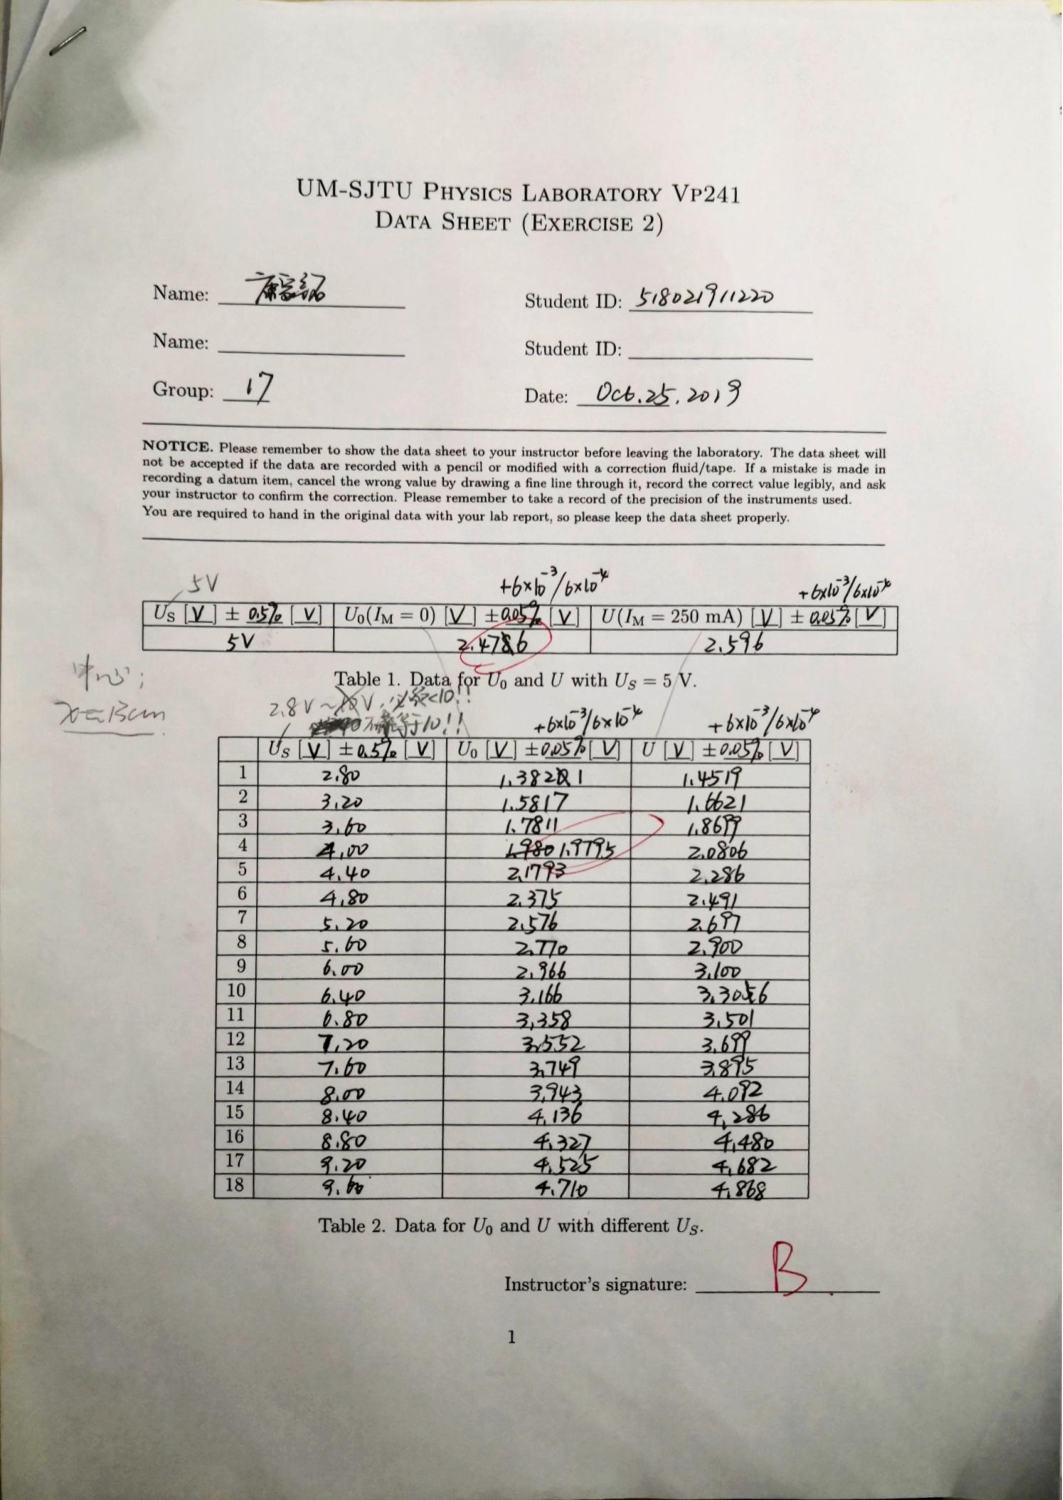
\includepdf[pages=-]{lab2datasheet.pdf}

\end{document}
